%!TEX root = lab3.tex

\setcounter{chapter}{2}
\chapter{\acs{ipv4} and \acs{ipv6}}

What you will learn in this lab:
\begin{itemize}
	\item Differences between \acs{ipv4} and \acs{ipv6}.
	\item What the effect is of netmasks.
	\item Differences in fragmentation.
	\item How \ac{nat} works.
	\item How \ac{dhcp} works.
\end{itemize}

\newpage
\section{Lab 3}\label{sec:lab3}
Lab 3 covers the differences between \acs{ipv4} and \acs{ipv6}. This lab is divided in parts where each part compares an \acs{ipv4} feature to its \acs{ipv6} counterpart. You will need to build a dual stacked setup meaning every host runs both versions of \acs{ip}.

\subsection{Netmasks}

In this part of the lab you explore the effects of changing the netmask of an interface.

\begin{exercise}{Netmasks}
	\begin{figure}[ht]
		\centering
		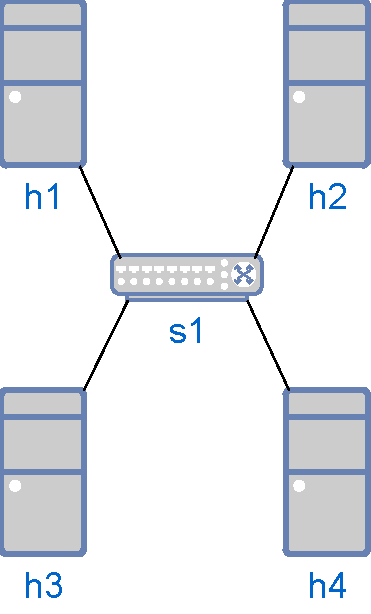
\includegraphics[width=.2\linewidth]{graphics/Lab3-Network1}	
		\caption{Network configuration for part 1.}
		\label{fig:lab3-network1}
	\end{figure}
\begin{table}[h!t]
\centering
\begin{tabular}{| c | c | c |}
    \hline
    \textbf{Linux} PC & \textbf{IPv6 address} & \textbf{IPv4 address} \\
    \hline
    h1 & \texttt{fc00::1/48} & \texttt{10.0.0.1/8} \\
    h2 & \texttt{fc00::2/64} & \texttt{10.0.0.2/24} \\
    h3 & \texttt{fc00:0:0:1::3/48} & \texttt{10.0.255.3/16} \\
    h4 & \texttt{fc00:0:0:1::4/64} & \texttt{10.1.0.4/24} \\
    \hline
\end{tabular}
\caption{IP addresses and subnet masks}
\label{tab:lab2-part7-addresses}
\end{table}

\begin{enumerate}
\item Write a python script that creates the topology shown in figure and table \ref{fig:lab3-network1} and save it to \file{py}.
\item Open an \incommand{xterm} on s1 and start a wireshark session on the \incommand{s1} interface. This will capture all packets that go through the switch (from all hosts).
\item Issue the \incommand{pingall} command in mininet.
\item Save the Wireshark trace to \file{pcapng}. Save the output of the pingall command to \file{ping.txt}.
\end{enumerate}

\textbf{Use the data captured with Wireshark in \linktrace[1]{pcapng} and the output in \linktrace[1]{ping.txt} to answer the questions. Support your answers with the saved Wireshark data.}

\question{Use the output from the pingall and the Wireshark trace file (by referring to packet numbers) to explain what happened for each of the ping commands. Were all pings successful? For all pings (successful or not), explain why.}{2}
\end{exercise}

\newpage
\subsection{Fragmentation in \acs{ipv4} and \acs{ipv6}}

Figure \ref{fig:lab3-network2} shows the network setup for this part of the lab. There are two different subnets which are connected by r1. Note that \acs{ip} addresses are given for both \acs{ip} versions.

\begin{figure}[ht]
	\centering
	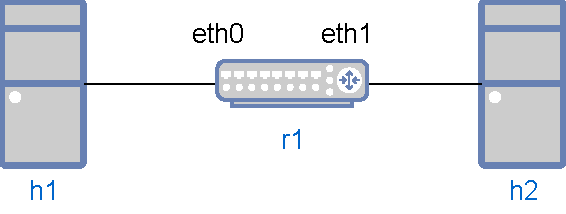
\includegraphics[width=.5\linewidth]{graphics/Lab3-Network2}	
	\caption{Network configuration for part 2.}
	\label{fig:lab3-network2}
\end{figure}

\begin{table}[h!t]
	\centering
	\begin{tabular}{| c | l | l |}	
		\hline
		\textbf{hosts} & \textbf{Interface eth0} & \textbf{Interface eth1} \\ \hline
		\multirow{2}{*}{h1} & \ipaddr{fc00:0:0:1::1/64} & \multirow{2}{*}{N/A} \\ 
		& \ipaddr{10.0.1.1/24} & \\ \hline
		\multirow{2}{*}{r1} & \ipaddr{fc00:0:0:1::10/64} & \ipaddr{fc00:0:0:2::10/64} \\
		& \ipaddr{10.0.1.10/24} & \ipaddr{10.0.2.10/24} \\ \hline
		\multirow{2}{*}{h2} & \ipaddr{fc00:0:0:2::2/64} & \multirow{2}{*}{N/A} \\ 
		& \ipaddr{10.0.2.2/24} & \\
		\hline
	\end{tabular}
	\caption{\acs{ip} addresses of all PCs for part 2.}
	\label{tab:lab3-network2}
\end{table}

In this part of the lab, you observe the differences in \acs{ip} Fragmentation. In the previous lab, you have already observed how fragmentation has an effect of the overall throughput of a connection. In this lab, you will take a look of how fragmentation is done differently in \acs{ipv4} and \acs{ipv6}.

\begin{exercise}{\acs{udp} and Fragmentation}
In this exercise you observe \acs{ip} fragmentation of \ac{udp} traffic. In the following exercise, use \incommand{iperf} to generate \ac{udp} traffic between h1 and h3, across \acs{ip} router r1.

\remark This is one of the few exercises where you \textbf{must use iperf instead of iperf3}. Read up on the man page of iperf as the syntax is slightly different from iperf3!

\remark If you want to redo this exercise, you should stop mininet and restart it, or you have to make sure the path \acs{mtu} cache is empty on h1. You can clear the cache with \incommand{ip (-6) route flush cache}. You can see the cached path \acs{mtu} with \incommand{ip (-6) route get [IP address]}

\begin{enumerate}
	\item Write a python script to form the network as shown in Figure \ref{fig:lab3-network2} and Table \ref{tab:lab3-network2} and save it to \file{py}.
	\item Change the \acs{mtu} on r1-eth1 to 1280 bytes.
	\item Execute the following command on h1: \verb!echo 1 > /proc/sys/net/ipv4/ip_no_pmtu_disc!
	\item Start Wireshark on the eth0 and eth1 interfaces of r1 and start to capture traffic. Do not set any filters.
	\item Use \incommand{iperf} to generate \ac{udp} traffic \textbf{over \acs{ipv6}} between h1 and h2. Configure the \incommand{iperf} client to send 2 seconds of traffic to the server.
	\item Repeat the previous step, but this time use \acs{ipv4}.
	\item Stop the traffic captures on r1 and save the Wireshark output to \file{eth0.pcapng} and \file{eth1.pcapng}.
	\item Now, execute the following on h1: \verb!echo 0 > /proc/sys/net/ipv4/ip_no_pmtu_disc!
	\item Start Wireshark on the eth0 and eth1 interfaces of r1 and start to capture traffic. Do not set any filters.
	\item Use \incommand{iperf} to generate \ac{udp} traffic \textbf{over \acs{ipv4}} between h1 and h2. Configure the \incommand{iperf} client to send 2 seconds of traffic to the server.
	\item Stop the traffic captures on r1 and save the Wireshark output to \file{eth0.pmtu.pcapng} and \file{eth1.pmtu.pcapng}.
\end{enumerate}

\textbf{Use the data captured with Wireshark in \linktrace[1]{eth0.pcapng}, \linktrace[1]{eth1.pcapng}, \linktrace[1]{eth0.pmtu.pcapng} and \linktrace[1]{eth1.pmtu.pcapng} to answer the questions. Support your answers with the saved Wireshark data.} The first questions are only about the first two Wireshark traces. It will be clearly stated when you need to look at the second set of Wireshark trace files.

\question{Both \acs{udp} streams in the first part of the exercise were fragmented. What differences (regarding fragmentation) do you see between \acs{ipv4} and \acs{ipv6}?}{1}
\question{Why is it important that the path \acs{mtu} cache was empty for this experiment? What would be different in the case of \acs{ipv6} if we did the experiment twice in a row without clearing the cache? What about \acs{ipv4}?}{1}
\question{Identify which fields in the header(s) are used for fragmentation in \acs{ipv4}.}{1}
\question{Identify which fields in the header(s) are used for fragmentation in \acs{ipv6}.}{1}
\question{Compare the amount of bytes that are needed for fragmentation in both \acs{ip} protocols. Consider the overhead when fragmentation is needed and when it is not needed.}{1}
\question{\acs{ipv4} allows fragmentation in intermediate routers where \acs{ipv6} forbids this. However, \acs{ipv4} can also perform end-to-end fragmentation. This is what happened in the last part of the exercise, where you saved the second set of Wireshark trace files. Take a look at those last trace files, and compare them to the first set (only look at \acs{ipv4}). What difference(s) regarding fragmentation do you see when you compare both iperf sessions? }{1}
\question{Compare the way \acs{ipv4} performs end-to-end fragmentation to the way this is done in \acs{ipv6}. What are the differences and similarities?}{1}
\question{What do you think is the main advantage of not allowing intermediate hosts to fragment \acs{ipv4} packets?}{1}
\end{exercise}

\newpage
\subsection{\acs{nat}, \acs{dhcp} and Router Advertisements}

In this part we set up \ac{nat}, \ac{dhcp} and router advertisements. These protocols are used to simplify network configurations. \acs{dhcp} and router advertisements are used to automatically configure clients when they connect to a network. \acs{nat} is used to conserve \acs{ipv4} addresses.

\subsubsection{\acf{dhcp}}

The \acf{dhcp} can be used to dynamically set and change configuration parameters of Internet hosts, including \acs{ip} address, subnet mask, default router, and \ac{dns} server. \ac{dhcp} is based on a client-server model. \ac{dhcp} clients send requests to a \ac{dhcp} server and the server responds with an allocation of \acs{ip} addresses and other configuration parameters.

A \ac{dhcp} client is assigned an \acs{ip} address for a limited period of time, which is called a lease. Information on current leases is stored at both the client side and the server side.

On a Linux system, a \ac{dhcp} server is started with the command \incommand{dhcpd}. The \ac{dhcp} server reads the configuration file \path{/etc/dhcp/dhcpd.conf}. The configuration file contains information on available \acs{ip} addresses, and other configuration information. The following is an example of a configuration file for a \acs{dhcp} server:
\begin{framed}
\begin{Verbatim}[gobble=1,formatcom=,fontfamily=courier,fontseries=,frame=none,numbers=none]
	#dhcpd.conf file
	default-lease-time 600;
	
	subnet 10.0.0.0 netmask 255.0.0.0 {
		range 10.0.100.0 10.0.255.255; 
		option routers 10.0.0.1; 
		default-lease-time 120;
	}
\end{Verbatim}
\end{framed}

The \ac{dhcp} client is assigned an \acs{ip} address for a period of time that is known as a lease. The above configuration file assigns \acs{ip} addresses for a lease time of 600 seconds (default-lease- time). For requests on network \ipaddr{10.0.0.0/8}, the \ac{dhcp} server assigns \acs{ip} addresses in the range \ipaddr{10.0.100.0 - 10.0.255.255}, assigns \ipaddr{10.0.0.1} as the default gateway, and limits the lease of addresses to 120 seconds, thus, overruling the global limit of 600 seconds.

Starting a \ac{dhcp} client on a host (e.g. h1) is simple. It can be done with one command: \incommand{dhclient h1-eth0}.

However, because all the (virtual) hosts created by ipmininet share the same underlying file system, when you have multiple virtual hosts all running \incommand{dhclient}, they would all start to use the same leases file and PID file simultaneously. This should be avoided. In order to do so, some optional parameters should be added to the \incommand{dhclient} command:
\begin{description}
	\item[\incommand{-lf <leases\_file>}] to use a different client leases file on each virtual host.
	\item[\incommand{--no-pid}] to disable using a PID file.
\end{description}

\remark The exact same parameters can (and should!) also be used on any host running a \incommand{dhcpd} server. This way, it is 100\% sure you are performing the experiment without having stale files from previous attempts (or from concurrently running dhcp servers).

\remark Don't forget to add these extra parameters when you are performing the next exercises!

\begin{exercise}{\ac{dhcp} Setup}
	\begin{figure}[ht]
		\centering
		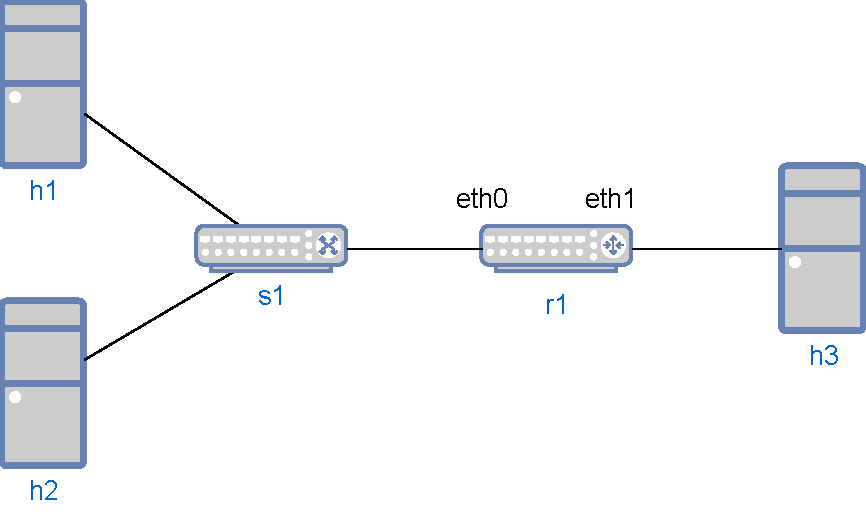
\includegraphics[width=.6\linewidth]{graphics/Lab3-Network3}	
		\caption{Network configuration for part 3.}
		\label{fig:lab3-network3}
	\end{figure}
	
	\begin{table}[h!t]
		\centering
		\begin{tabular}{| c | l | l |}	
			\hline
			\textbf{hosts} & \textbf{Interface eth0} & \textbf{Interface eth1} \\ \hline
			h1 & N/A & N/A \\ \hline
			h2 & N/A & N/A \\ \hline
			\multirow{2}{*}{r1} & \ipaddr{fc00:0:0:1::1/64} & \ipaddr{fc00:0:0:2::1/64} \\
			& \ipaddr{10.0.1.1/24} & \ipaddr{10.0.2.1/24} \\ \hline
			h3 & N/A & N/A \\ \hline
		\end{tabular}
		\caption{\acs{ip} addresses of all PCs for part 3.}
		\label{tab:lab3-network3}
	\end{table}
\begin{enumerate}
	\item Write a python script that results in the topology shown in figure \ref{fig:lab3-network3} and table \ref{tab:lab3-network3} and save it to \file{py}.
	\item We want to analyze packets used for DHCP configuration. Start to capture traffic with Wireshark on interface eth0 of r1.	
	\item Configure r1 as a \acs{dhcp} server:
	\begin{enumerate}
		\item On r1, set up a configuration file so that \acs{ip} addresses are assigned as follows:
		\begin{itemize}[noitemsep,nolistsep]
			\item The default and maximum lease time should be 2 minutes.
			\item On network \ipaddr{10.0.1.0/24}, \acs{ip} addresses are assigned in the range \ipaddr{10.0.1.50 - 10.0.1.100} with default gateway \ipaddr{10.0.1.1} and \ac{dns} server \ipaddr{8.8.8.8}.
			\item On network \ipaddr{10.0.2.0/24}, \acs{ip} addresses are assigned in the range \ipaddr{10.0.2.50 - 10.0.2.100} with default gateway \ipaddr{10.0.2.1} and \ac{dns} server \ipaddr{8.8.8.8}.
		\end{itemize}
		Save the configuration file to \path{/home/computernetwerken/dhcpd.conf}
		\item Make sure the file \path{/home/computernetwerken/dhcpd.leases} exists. It can be an empty file.	
		\item Open a \incommand{xterm} on r1, and start the \ac{dhcp} server by typing:
		\begin{cmdblock}[gobble=3]
			r1% dhcpd -f --no-pid -cf /home/computernetwerken/dhcpd.conf \\
			-lf /home/computernetwerken/dhcpd.leases
		\end{cmdblock}
		The \ac{dhcp} server daemon listens for requests from \ac{dhcp} clients on all its interfaces. In Linux, the \ac{dhcp} server must be restarted each time the configuration file is modified. Since only one \ac{dhcp} server can run at a time, you may need to terminate the current \ac{dhcp} server process.
	\end{enumerate}
	\item Start \ac{dhcp} clients on h1, h2 and h3 with the command:
	\begin{cmdblock}[gobble=2]
		% dhclient hX-eth0 --no-pid -lf /home/computernetwerken/hX.dhclient.leases
	\end{cmdblock}
	\item Use the commands \incommand{ifconfig} and \incommand{route -4 -n} to see if the automatic configuration is successful on all hosts. Verify with a \incommand{pingall} all hosts can reach each other.
	\item Stop the Wireshark capture. Save it to \file{pcapng}.
	\item Make sure you include the dhcp server configuration file in the \path{/traces} folder of your lab report.
\end{enumerate}
	
\textbf{Use the data captured with Wireshark in \linktrace[1]{pcapng}, to answer the questions. Support your answers with the saved Wireshark data.}

\question{Which \acs{ip} addresses are assigned to h1 and h2?}{1}
\question{Observe and interpret the different \ac{dhcp} packets. What is their purpose?}{1}
\question{Identify and interpret all option fields in the \ac{dhcp} packet types that you observe.}{1}
\question{Observe the source and destination \acs{ip} addresses of the packets that are sent between \ac{dhcp} client and \ac{dhcp} server.}{1}
\question{How is it possible that a host can send and receive \ac{dhcp} packets, even though it does not have an \acs{ip} address?}{1}
\question{In most client-server applications, the port number of a server is a well-known number (e.g., an HTTP server uses port number 80, an ssh server uses port number 22, etc.), while the client uses a currently available (random) port number. \ac{dhcp} is different. Here, both the client and the server use a well-known port: \acs{udp} port 67 for the \ac{dhcp} server, and \acs{udp} port 68 for the \ac{dhcp} client. Refer to RFC 2131 and provide an explanation for this protocol design choice.}{1}


\end{exercise}

\begin{exercise}{\ac{dhcp} leases}
	
In this exercise you will see what happens when a client can't reach the \ac{dhcp} server anymore. We will simulate this by disabling the \ac{dhcp} server on r1.
	
\begin{enumerate}
	\item Start the script from the previous exercise, and make sure all hosts get an \acs{ip} address from the \acs{dhcp} server.
	\item Wait until every host has renewed their lease at least once. This cannot take longer than 120 seconds.
	\item Start to capture traffic with Wireshark on interface eth0 and eth1 of r1. You can select both interfaces simultaneously in Wireshark so all data is stored in a single \incommand{pcapng} file.
	\item Stop the \ac{dhcp} server (Ctrl-C).
	\item Watch what the clients do when they try to renew their leases. Wait at least 3 minutes. After this the clients should no longer have an \acs{ip} address.
	\item After the clients have lost their IP address, stop the Wireshark capture and save it to \file{pcapng}.
	\item Make sure to include a copy of the dhcp server leases file, as well as the dhcp client leases file from all hosts in your report!
\end{enumerate}

\textbf{Use the data captured with Wireshark in \linktrace[1]{pcapng}, to answer the questions. Support your answers with the saved Wireshark data.}

\question{Why does a \ac{dhcp} server have a leases file? What is it used for?}{1}
\question{Explain the entries in the client lease file.}{1}
\question{What attempts did the clients make to renew their leases? You should notice two stages. What happens during those two stages? What happens afterwards (i.e. after the renewal fails)?}{1}

\end{exercise}

\subsubsection{\acf{nat}}

\acf{nat} refers to a function that replaces the \acs{ip} addresses (and possibly the port numbers) of \acs{ip} datagrams. \ac{nat} is run on routers that connect private networks to the public Internet, to replace the \acs{ip} address-port pair of an \acs{ip} packet with another \acs{ip} address-port pair. Generally, the operations of \ac{nat} are specified in terms of a set of rules which determines how \acs{ip} addresses are to be replaced.

Often, a \ac{nat} device is referred to as a \ac{nat} box. One of the reasons for using \ac{nat} is that it conserves \acs{ip} addresses. \ac{nat} allows hosts in a private network to share public \acs{ip} addresses, or to limit the use of public \acs{ip} addresses to a small number of hosts in the private network.

Private networks may have \acs{ip} addresses that are non-Internet routable, as specified in RFC 1918. This means that the Internet routers do not have entries in their routing tables for these addresses.

In the following exercise, we consider a special use of \ac{nat} that allows multiple private \acs{ip} addresses to be mapped to a single public \acs{ip} address. This use of \ac{nat} is called \acs{ip} masquerading, port address translation (PAT) or Network Address and Port Translation (NAPT). Here, the private network has only a single public \acs{ip} address, but has multiple hosts in the private network. \acs{ip} Masquerading modifies the port number of packets so that the single public \acs{ip} address can be overloaded.

The Linux kernel on all PCs has been built with netfilter, which adds the ability to set \acs{ip} packet filters in a Linux system. \acs{ip} packet filters are used to add firewalls as well as \ac{nat} functionality to a system. The \incommand{iptables} command is used to set up, maintain, and inspect \acs{ip} packet filter rules to a Linux kernel:

On a Linux system, the configuration of \ac{nat} manipulates a set of rules of the netfilter utility, called \ac{nat} table. The rules in the \ac{nat} table are grouped in so- called chains. Two of the built-in chains are called \texttt{PREROUTING} and \texttt{POSTROUTING}:
\begin{framed}
\begin{description}
	\item[\texttt{PREROUTING}] \hfill \\
		The rules in this chain are applied to incoming datagrams.
	\item[\texttt{POSTROUTING}] \hfill \\
		The rules in this chain are applied to outgoing datagrams. The main rule is S\ac{nat} (Source Network Address Translation), which specifies how the source address of an outgoing \acs{ip} datagram should be modified.
\end{description}
\end{framed}

Commands that manipulate the \ac{nat} table start with \incommand{iptables -t nat}. The following are some of the most important commands that manipulate the \ac{nat} table:
\begin{framed}
	\begin{description}
		\item[\texttt{iptables -t nat -L}] \hfill \\
			Displays all rules in the \ac{nat} table
		\item[\texttt{iptables -t nat -F POSTROUTING}] \hfill \\
			Deletes all rules in the \texttt{POSTROUTING} chain of the \ac{nat} table
		\item[\texttt{iptables -t nat -A POSTROUTING -j S\ac{nat} -{}-to IPAddr -s PrivateIPAddr/netmask}] \hfill \\
			Adds the following rule to the \texttt{POSTROUTING} chain of the \ac{nat} table: ``In \acs{ip} datagrams that go to the public network, the \acs{ip} source address PrivateIPAddr/netmask is changed to IPAddr''.\\
			Example: The source address of outgoing \acs{ip} datagrams that match ``10.0.1.0/24'' is changed to 128.195.7.32.\\
			\incommand{iptables -t nat -A POSTROUTING -j SNAT -{}-to 128.195.7.32 -s 10.0.1.0/24}
	\end{description}
\end{framed}


\begin{exercise}{A \ac{nat} setup}
In this exercise, we use the same topology as in figure \ref{fig:lab3-network3}, and r1 will be configured as a \ac{nat} router. Configure the topology to use the \acs{ipv4} addresses as shown in the table below (note we are only using \acs{ipv4} in this exercise).

\begin{table}[h!t]
	\centering
	\begin{tabular}{| c | l | l |}	
		\hline
		\textbf{hosts} & \textbf{Interface eth0} & \textbf{Interface eth1} \\ \hline
		h1 & 10.0.1.101/24 & N/A \\ \hline
		h2 & 10.0.1.102/24 & N/A \\ \hline
		r1 & 10.0.1.1/24 & 128.66.0.1/24 \\ \hline
		h3 & 128.66.0.103/24 & N/A \\ \hline
	\end{tabular}
	\caption{\acs{ip} addresses of all PCs for exercise 5.}
	\label{tab:lab3-network3-ex5}
\end{table}
%net["h1"].cmd("ethtool -K h1-eth0 tso off")
\begin{enumerate}
	\item Write a script that sets up the correct topology and save it to \file{py}.
	\item On r1, add a rule to the \ac{nat} table so that the \acs{ip} source address of outgoing \acs{ip} datagrams from network \ipaddr{10.0.1.0/24} are set to \acs{ip} address \ipaddr{128.66.0.1}. By doing this you turn the \ipaddr{10.0.1.0/24} network into a private network that uses r1 to communicate with the public network (\ipaddr{128.66.0.0/24}).
	\item On h3, execute the following command: \incommand{ip route del default via 128.66.0.1}. This is necessary, as mininet doesn't make a distinction between ``private'' addresses that will be NATed, and ``public'' addresses. If h3 would set its default router to r1, packets would be routed normally, as usual, but in this case, this needs to be avoided.
	\item Observe traffic at a \ac{nat} device:
	\begin{enumerate}
		\item To observe the \acs{ip} address translation, capture packets on both interfaces of r1.
		\item Start up the \incommand{/sbin/sshd} server on h1, h2, r1 and h3.
		\item Establish a set of ssh sessions. Try to create following sessions (there is no need to log in; you can CTRL-C at the login prompt) and see which ones are successful:
		
		\begin{tabular}{|l}
			h1 $\rightarrow$ h2 \\
			h1 $\rightarrow$ h3
		\end{tabular} \\
	
		\begin{tabular}{|l}
			h2 $\rightarrow$ r1 (eth0) \\
			h2 $\rightarrow$ h3
		\end{tabular} \\
	
		\begin{tabular}{|l}
			h3 $\rightarrow$ r1 (eth1) \\
			h3 $\rightarrow$ h1
		\end{tabular}

		Note which ssh commands succeed. You will need this information to answer the questions.
		\item Generate traffic between h1 and h3 and between h2 and h3 at the same time. You can do this by establishing an ssh session between these hosts, logging in (with as username \emph{computernetwerken}, and as password \emph{mvkbj1n}), and maybe type some simple commands. 
		\item Also issue a ping command from h1 to h3, and, simultaneously, from h2 to h3. Make sure you have some pings that are sent in both sessions, and the stop both pings.
	\end{enumerate}
	\item Save the Wireshark data to \file{eth0.pcap} and \file{eth1.pcap}.
\end{enumerate}

\textbf{Use the data captured with Wireshark in \linktrace[1]{eth0.pcap} and \linktrace[1]{eth1.pcap} the questions. Support your answers with the saved Wireshark data.}

\question{For each of the \incommand{ssh} commands above, provide an explanation why a command succeeds or fails.}{1}
\question{Explain how r1 knows which ssh packets should be forwarded to h1 and which ssh packets should be forwarded to h2.}{1}
\question{Explain how r1 knows which ping packets should be forwarded to h1 and which ping packets should be forwarded to h2.}{1}
\question{Multiple hosts using the same \acs{ip} address (i.e. behind a \acs{nat}) can be troubling in some situations like \acs{ip} ban and traceability of suspicious traffic. Explain the impact of using \ac{nat} in these scenarios.}{1}

\end{exercise}

\subsubsection{Router Advertisements}

Like \acs{dhcp}, router advertisements can be used to dynamically set and change configuration parameters of Internet hosts. 

On a Linux system, a router advertisement daemon is started with the command \incommand{radvd}. The daemon by default reads the configuration file \path{/etc/radvd.conf}. However, using the \texttt{-C}  flag, an alternative location of the radvd configuration file can be passed on to the daemon. The configuration file contains information on available \acs{ip} addresses, and other configuration information. The following is an example of a configuration file:
\begin{framed}
\begin{Verbatim}[gobble=1,formatcom=,fontfamily=courier,fontseries=,frame=none,numbers=none]
	#radvd.conf file
	
	interface eth0 {
		AdvSendAdvert on;
		MaxRtrAdvInterval 30;
		prefix 2001:db8::/64 {
			AdvOnLink on;
			AdvAutonomous on;
			AdvRouterAddr off;
			AdvPreferredLifetime 60;
		};
		RDNSS 2001:4860:4860::8888 {};
	};
	
	interface eth1 {
		AdvSendAdvert on;
		MaxRtrAdvInterval 30;
		prefix 2001:db8:0:1::/64 {
			AdvPreferredLifetime 60;
		};
		RDNSS 2001:4860:4860::8888 {};
	};
\end{Verbatim}
\end{framed}

This config file will enable router advertisements on eth0 and eth1. The option ``AdvSendAdvert'' enables this. For each interface a prefix and a \acs{dns} server are specified. The configuration for eth0 and for eth1 are identical in this example. In the first case the parameters for the prefix are explicitly specified. For eth1, parameters with default values are omitted. ``AdvPreferredLifetime'' indicates how long the given prefix should be preferred by the host. When the prefix is not refreshed within this interval, another prefix may become preferred. The prefix remains valid for a period of ``AdvValidLifetime'' though.

\begin{exercise}{Router Advertisements on Linux PC}

For this exercise, you once again start from the same toplogy as in figure \ref{fig:lab3-network3}, but this time with the following IP addresses set:

\begin{table}[h!t]
	\centering
	\begin{tabular}{| c | l | l |}	
		\hline
		\textbf{hosts} & \textbf{Interface eth0} & \textbf{Interface eth1} \\ \hline
		h1 & N/A & N/A \\ \hline
		h2 & N/A & N/A \\ \hline
		r1 & \ipaddr{fc00:0:0:1::1/64} & \ipaddr{fc00:0:0:2::1/64} \\ \hline
		h3 & N/A & N/A \\ \hline
	\end{tabular}
	\caption{\acs{ip} addresses of all PCs for part 3.}
	\label{tab:lab3-network3}
\end{table}

\begin{enumerate}
	\item Write a script that results in the correct topology and save it to \file{py}.
	\item Start to capture traffic with Wireshark on interface eth0 of r1.
	\item Configure r1:
	\begin{enumerate}
		\item On r1, create up a \incommand{radvd} configuration file so it distributes the correct prefixes and assigns a \acs{dns} server as shown in the example. Save it to \file{conf}
		\item On r1, start the router advertisements daemon (run the \incommand{radvd -C L3-6-1.conf} command).
	\end{enumerate}

	\item Use the commands \incommand{ip -6 addr show} and \incommand{route -6 -n} to see if the automatic configuration is successful on all hosts. Every host should be able to ping all other hosts on their global \acs{ipv6} address at this point. Issue a ping from h1 to h3 and from h3 to h2.
	\item Bring the interface eth0 of h2 down and back up:
	\item Now shut down the router advertisements daemon on r1 with \incommand{pkill}
	\item Wait at least 60 seconds while watching the \acs{ip} address and route configuration of eth0 on h1 (hint: use the \incommand{watch} command).
	Once this changes, save the result to \file[5]{h1.txt}.
	\item Stop the Wireshark capture and save it to \file{pcapng}.
\end{enumerate}

\textbf{Use the data captured with Wireshark in \linktrace[1]{pcapng} to answer these questions.  Support your answers with the saved Wireshark data.}

\question{Identify a router advertisement in the Wireshark capture. Which ICMP Options do you see? For each option, explain what it is used for.}{1}
\question{What is the destination \acs{ip} address of a router advertisement?}{1}
\question{After resetting interface eth0 of h2 you should have seen a router solicitation packet. What was the destination \acs{ip} address of this packet?}{1}
\question{The router responded to the solicitation with a router advertisement. What destination \acs{ip} address was used and why?}{1}
\question{After 60 seconds, the preferred lifetime of the prefix expires. How do you see this and what does this mean? Use the output saved in \linktrace{h1.txt}.}{1}
\question{Explain how hosts get a global \acs{ipv6} address based on the information in the router advertisement.}{1}
\question{Why doesn't the router advertisement daemon keep track of its hosts like an \acs{ipv4} \acs{dhcp} server?}{1}

\end{exercise}

\subsubsection{\acs{ipv6} Privacy Extension}

Privacy was not a pressing matter when the \acs{ipv6} standard was proposed in 1995. Later on, a \acs{ipv6} privacy extension was proposed in RFC 4941. 

\begin{exercise}{\acs{ipv6} privacy extension}
This exercise will demonstrate how and when Linux PCs use the privacy extension. They will generate random globally unique \acs{ipv6} addresses based on the prefix information in router advertisements.
	
\begin{enumerate}
	\item Re-use the previous setup.
	\item Change the settings \texttt{temp\_prefered\_lft} and \texttt{temp\_valid\_lft} to 60 seconds on h1, h2 and h3.
	\begin{cmdblock}[gobble=2]
		% echo 60 > /proc/sys/net/ipv6/conf/hX-eth0/temp_prefered_lft
		% echo 60 > /proc/sys/net/ipv6/conf/hX-eth0/temp_valid_lft
	\end{cmdblock}
	Normally these timers are much longer. We lower them here to demonstrate what happens when they expire.
	\item Enable the privacy extension on h1, h2 and h3 by writing a 2 to the configuration file \path{use_tempaddr}:
	\begin{cmdblock}[gobble=2]
		% echo 2 > /proc/sys/net/ipv6/conf/hX-eth0/use_tempaddr
	\end{cmdblock}
	Writing a 2 to this file enables the generation and use of a random address.
	\item Start capturing packets on the eth0 interface of r1.
	\item Start the router advertisements daemon on r1.
	\item You should see that the hosts each get a new \acs{ipv6} address when they receive a router advertisement. Use the command \incommand{ip -6 addr show} to verify this.
	\item Set up a continuous ping from h2 to h3. Use the global \acs{ipv6} address of h3 (\emph{not} the temporary address).
	\item At the same time open a ssh session from h2 to h3 (use the same global address). Generate traffic over this session. You can use the watch command for example:
	\begin{cmdblock}[gobble=2]
		% watch date
	\end{cmdblock}
	\item Wait at least 60 seconds and observe what happens. After that, stop the Wireshark capture and save it to \file{pcapng}.
\end{enumerate}

\remark An session that doesn't respond can be terminated with \incommand{pkill ssh}.
	
\textbf{Use the data captured with Wireshark in \linktrace[1]{pcapng}, to answer the questions. Support your answers with the saved Wireshark data.}

\question{Which of its \acs{ip} addresses does h2 use as source address for the ping? And which one for the ssh session?}{1}	
\question{Explain what you observed concerning the ping.}{1}
\question{Explain what you observed concerning the ssh session.}{1}
\question{What is different between the ssh session and the ping command?}{2}
\question{What is the purpose of the privacy extension? What potential privacy violation does it prevent.}{1}

\end{exercise}

